\chapter{Аналитический раздел}\label{sec:analyth}
В разделе описан способ выражения эмоций в тексте и подходы к его анализу. Приведены существующие размеченные корпуса для русского языка и описаны шкалы оценки тональности. Описано существующее решение для англоязычной лексики и рассмотрены некоторые модели данных, применяемые в no-SQL системах.  
\section{Подходы к анализу эмоций в тексте}
Лексическая тональность выражается в тексте на уровне лексем или коммуникационных фрагментов. Коммуникативные фрагменты -- это отрезки речи различной длины, которые хранятся в памяти говорящего в качестве стационарных частиц его языкового опыта и которыми он оперирует при создании и интерпретации высказываний. \cite{Гаспаров1996} Тональность текста в целом определяется лексической тональностью единиц, составляющих текст и правилами их сочетания.

Традиционный подход к определению эмоциональной оценки текста чаще всего заключается в использовании одномерного эмотивного пространства: позитив-негатив, то есть хорошо-плохо. Тональность текста определяется тремя факторами: субъектом тональности, тональной оценкой и объектом тональности. \cite{Пазельская2011}. Под субъектом тональности понимается автор высказывания, под объектом тональности -- объект, о котором высказывается субъект и под тональной оценкой -- эмоциональное отношение автора к такому объекту. 

Лексический уровень языковой системы характеризуется разнообразием экспрессивных слов. Однако, их денотация может изменяться в зависимости от культурного фона или географического положения. 
\subsection{Мониторинг индекса настроений}
Лексический фон вбирает в себя те ассоциативные сведения, которые накапливаются у носителей языка в процессе применения слова. \cite{МатвееваТ.2013} Соотвественно, аппроксимация оценки экспрессивного слова неразрывно связана с регионом, в котором проживает субъект тональности. 
 
В работе \cite{ЩекотинЕ.2020} исследовалась субъективная оценка благополучия, основанная на данных ВКонтакте об активности пользователей. Для формирования выборки были предложены критерии, приведенные ниже. 
\begin{enumerate}
	\item Географическая репрезентативность. Регионы представлены равномерно на всей территории РФ — все федеральные округа, все климатические и культуро-исторические зоны.
	\item Социально-экономическая репрезентативность. Согласно типологии \cite{Zubarevich2013}, населенные пункты были поделены по уровню социально-экономического развития на четыре типа, представленных ниже.
	\begin{enumerate}
		\item Крупные города -- Москва и города-миллионники, города с населением свыше 500 тыс. человек.
		\item  Средние по размеру индустриальные города с населением от 20 до 25 -- 300 тыс. человек.
		\item <<Периферия>> -- деревни, сёла и небольшие города.
		\item Республики Северного Кавказа и Юга Сибири.
	\end{enumerate}
\end{enumerate}
Результаты исследования показали существенную разницу между регионами России. Например, индекс социального (не)благополучия в Республике Алтай составил $-0,4632$, а в Алтайском крае $-18,2462$. Такая существенная разница, скорее всего, будет влиять на общий уровень энтузиазма, и, в результате, на измерение оценки тональных прилагательных. 
При подготовке обучающего набора данных следует уделить особое внимание разметке корпусов в соответствии с личными характеристиками субъекта -- пол, возраст, географическое положение и т.\,п.

В настоящее время результаты анализа онлайн-текстов не могут рассматриваться как полноценная альтернатива классическим подходам оценки мнений на основе массовых опросов. \cite{Дудина2017} Для получения более точных результатов автоматического извлечения тональности требуются заранее подготовленные данные -- размеченный словарь эмоций или размеченный корпус. Разметка должна предполагать не только обобщение данных до боле крупных групп населения (например, согласно типологии \cite{Zubarevich2013}), но и ассоциировние с социально-демографическими группами, учет пола и возраста.
\subsection{Шкалы оценки тональных слов}
В большинстве случаев для оценки тонального слова используется одномерная шкала (\ref{fig:scale:flat}).  

\begin{figure}[H]
	\centering
	
	\subfloat[]{%
		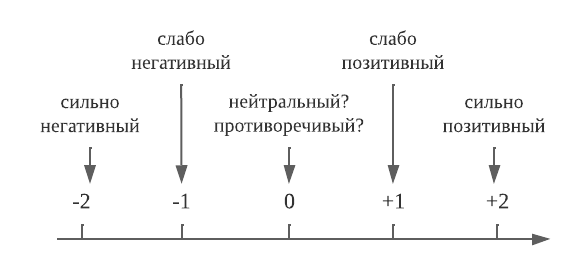
\includegraphics[width=0.7\textwidth]{assets/scale-flat.png}%
		\label{fig:scale:flat}
	} \newline
	\subfloat[]{%
		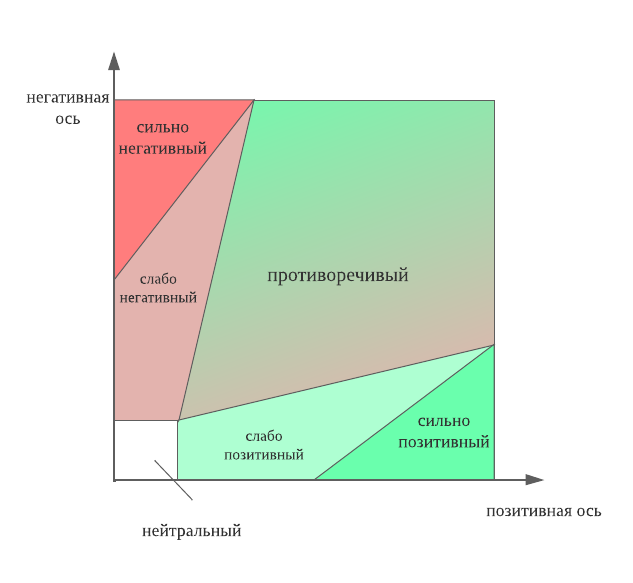
\includegraphics[width=0.7\textwidth]{assets/scale-thicc.png}%
		\label{fig:scale:thicc}%
	}
	\caption{Эмотивное пространство -- плоское(а), объемное(б)}
\end{figure}

На такой шкале расположены шесть классов оценки: <<сильно позитивный>>, <<слабо позитивный>>, <<сильно негативный>>, <<слабо негативный>>, <<нейтральный>> (отсутствие выраженного эмотивного окраса) и <<противоречивый>> (в равной мере присутствует негативный и позитивный эмотивный окрас). Однако,  в таком случае возникает неопределенность в отношении нулевого, <<центрального>> значения -- ноль на плоской шкале может обозначать как отсутствие эмотивного окраса, так и присутствие позитивного и негативного окраса в равной мере.

Для разрешения этой неопределенности в качестве шаклы оценки используется двумерное пространство, представленное на рис. \ref{fig:scale:thicc}.  Границы между классами изображены приблизительно, симметрия предположительна.

Минимальное количество классов в корпусе -- два (позитивный и негативный). \cite{КотельниковЕ.2021} Встречаются также случаи пятибальной шкалы оценивания, где <<3>> -- это центральное значение и десятибальной шкалы, где <<5>> -- это центральное значение.

\subsection{Существующие размеченные эмоциональные корпуса}
\textit{Корпус ROMIP-2012}. \cite{Chetviorkin2012} Чтобы составить коллекцию, один эксперт разметил отзывы на книги, фильмы и цифорвые камеры. Для проверки ответов систем тестовая коллекция поступила на оценку одному экспертам.  В их задачу входило отобрать из всех имеющихся постов  такие посты, которые релевантны заданным предметным областям, содержат оценку упоминаемых объектов, а также классифицировать отобранные посты по трем шкалам: двухбалльной (позитивный, негативный), трехбалльной (позитивный, негативный, удовлетворительный), пятибалльной (отлично, хорошо, средне, плохо, ужасно).

\textit{Корпус SentiRuEval-2015}. \cite{Loukachevitch2015} В 2015 году было проведено тестирование автоматического анализа тональности русскоязычных текстов. Исследование было разделено на две части. В рамках первой части участникам было предложено найти слова и выражения, обозначающие важные характеристики сущности (аспектные термины), и классифицировать их по тональности и обобщенным категориям. Разметка экспертом проводилась по четырехбалльной шкале (позитивный, негативный, противоречивый и нейтральный), далее была проведена проверка. Корпус для первой части состоял из отзывов на автомобили.

В рамках второго задания анализировался корпус публикаций из социальной сети <<Твиттер>>, разметка была проведена тремя экспертами. Для разметки была использована четырехбалльная шкала. 

\textit{Корпус RuSentiment}. Корпус составлен из публикаций социальной сети ВКонтакте. \cite{Rogers2018} Был размечен тремя экспертами по трехбалльной шкале -- позитивный, негативный и нейтральный. 

\textit{Корпус Kaggle Russian News Dataset}. Интернет-ресурс Kaggle \cite{kaggle} содержит корпус, составленный из новостей Казахстана на русском языке. Был размечен по трехбалльной шкале -- позитивный, негативный и нейтральный. Метод аннотации и ресурсы неизвестны. 

\textit{Корпус LinisCrowd}. PolSentiLex \cite{Koltsova2016} -- тональный словарь, ориентированный на тексты социальных медиа, разработанный в рамках сотрудничества с Лаборатории интернет-исследований (ЛИНИС) НИУ ВШЭ. Для него была сформирована коллекция документов, посвященных социально-политической тематике. В  качестве источника данных использовались записи блог-платформы Живой Журнал и социальной сети Фэйсбук. Далее был создан краудфандинговый веб-ресурс \cite{linis}, позволяющий добровольцам размечать слова и тексты онлайн, а исследователям и практикам – использовать результаты разметки. 

\textit{Корпус tweets}. Tweets \cite{Рубцова2012} -- русскоязычный корпус сообщений социальной сети <<Twitter>>. Является одним из немногих на данный момент корпусом текстов на общую тематику. Корпус был разделен на три класса: позитивно окрашенные, негативно окрашенные и нейтральные. Сбор и разметка сообщений производились с помощью специального скрипта и привлечения экспертов. 
При анализе корпуса была выявленна склонность использовать чаще ту или иную часть речи в зависимости от эмотивной окраски сообщения. 

\section{Формализация задачи}
Задача сводится к поиску экспертов. Входными данными в такой задаче является исходная коллекции данных, полученных из массового опроса, а выходными -- более крупные группы населения, состоящих из экспертов, обладающих определенной характеристикой. В такой задаче выделяют два основных подхода -- первый предполагает выполнение поиска экспертов в две стадии: первичный поиск документов в соответствии с пользовательским запросом и последующий поиск людей в найденных документах. \cite{Petkova2006} Второй подразумевает построение описания  для каждого человека, а поиск людей фактически производится в этих описаниях. \cite{Balog2006} Для рассматриваемой задачи требуется использовать второй подход.

Важная особенность модели -- это способ моделирования связи между лексикой и человеком. Такая связь выстраивается не только в зависимости от топологических особенностей автора в подсети термина. Здесь подсеть термина -- это граф, в котором узлы представляют собой людей, поставивших определенную отметку прилагательному. 

\section{Обзор существующего решения}
Британская международная компания <<YouGov>> провела исследование, в котором выявило, насколько различается численная оценка эмотивных прилагательных в зависимости от географического положения субъекта тональности. \cite{goodisgood} 
В рамках исследования <<YouGov>> продемонстрировали респондентам список эмотивных прилагательных и предложили оценить каждое из них по шкале 0-10, где 0 -- это <<сильно негативный>>, а 10 -- <<сильно позитивный>>. Результаты исследования изображены на рис. \ref{fig:gig-all}.

Исследование было проведено в двух странах - США и Великобритании. Исследование выявило, что респонденты из Великобритании более пессимистичны, чем респонденты из Штатов. В списке было 31 прилагательное, которое в среднем оценили на 8 из 10, но респонденты из Великобритании дали 28 из них более низкий балл. Однако, 9 самых позитивных прилагательных респонденты из Великобритании оценили более высоко. \\
\begin{center}
	\begin{figure}[H]
		\centering
		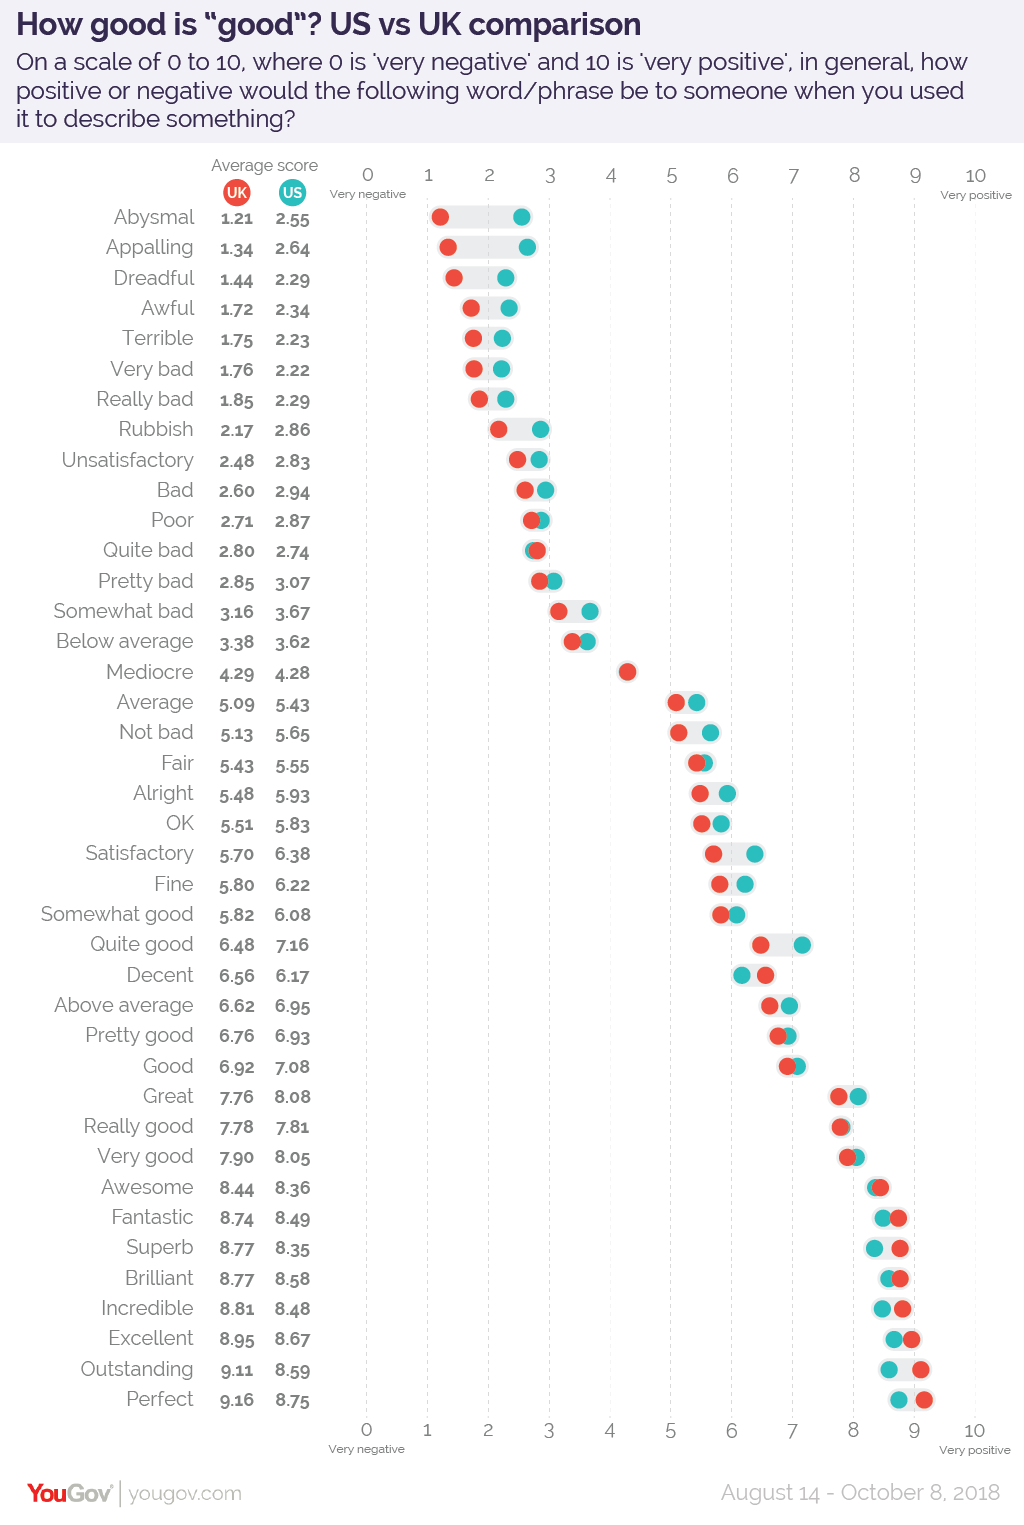
\includegraphics[width=0.85\linewidth]{assets/goodisgood-all.png}
		\caption{Результаты исследования <<YouGov>>\cite{goodisgood}}
		\label{fig:gig-all}
	\end{figure}
\end{center}
 
Самое большое различие наблюдается в более негативных прилагательных -- разрыв оценки в слове <<abysmal>> составляет 1.34 балла -- респонденты из Великобритании оценили на  1.21, из Штатов -- на 2.55. 

Похожие результаты наблюдаются и при оценке слова <<appalling>> -- респонденты из Штатов присвоили слову в среднем более высокую оценку, чем респонденты из Великобритании -- различие составляет 1.3 балла.

Самое небольшое различие наблюдается при оценке слова <<mediocre>> -- разница не дотягивает и до половины балла. В Штатах слово оценили на 4.28, а в Великобритании -- на 4.29.
\section{Использование нереляционных баз данных}
Нереляционные базы данных могут хранить неструктурированные данные в виде целостной сущности -- база данных NoSQL не накладывает ограничений на типы хранимых данных. Потребность в использовании нереляционной базы данных обусловлена тем, что данные, полученные в результате выявления объектов и связей между ними принадлежат классу, который находится <<между>> Data Mining и Text Mining -- Linked Objects mining(далее LOM-mining). \cite{Попов2004}
\subsection{Обзор моделей данных}
Существует множество моделей данных в нереляционных базах данных. \\
\textit{Колоночное хранилище}. В колоночных нереляционных базах данных данные хранятся в ячейках, сгруппированных в колонки, а не в строки данных. Колонки логически группируются в колоночные семейства. Колоночные семейства могут состоять из практически неограниченного количества колонок, которые могут создаваться во время работы программы или во время определения схемы. Чтение и запись происходит с использованием колонок, а не строк. \\
\textit{Система ключ-значение}. Представляет собой большую хэш-таблицу. Каждое значение сопоставляется с уникальным ключом, и хранилище ключей использует этот ключ для хранения данных, применяя к нему некоторую функцию хэширования. Выбор функции хэширования должен обеспечить равномерное распределение хэшированных ключей по хранилищу данных. \cite{nosql} \\
\textit{Документо-ориентированные базы данных}. Такие базы данных представляют собой усложненную систему <<ключ-значение>>, которая позволяет к каждому ключу привязывать вложенные данные. \\
\textit{Графовая модель} Графовые базы данных предназначены для хранения взаимосвязей и навигации в них. В графовых базах данных используются узлы для хранения сущностей данных и ребра для хранения взаимосвязей между сущностями. Для запросов, соответствующих графовой модели, поиск в такой базе может быть эффективнее, чем в реляционной. 

Ниже приведена таблица некоторых no-SQL баз данных.(\ref{tab:nosql-store}). 
\begin{table}[H]
	\centering
	\caption{Хранение данных в различных no-SQL базах данных}
	\renewcommand{\arraystretch}{1.5}
	\begin{tabular}{||c|c||}
		\hline
		\textit{База данных} & \textit{Модель данных} \\ \hline
		Cassandra & Семейства столбцов \\ \hline
		Redis & Ключ-значение \\ \hline
		MongoDB & Документо-ориентированая \\ \hline
		Neo4j & Графовая \\ \hline
		Scalaris & Ключ-значение \\ \hline
	\end{tabular}
	\label{tab:nosql-store}
\end{table}
Наиболее подходящими средствами для задачи LOM-mining можно назвать
методы из теории графов и теории множеств, \cite{Попов2004} поэтому наиболее подходящая модель хранилища данных -- графовая. 

\addsec{Вывод}
Были проанализированы некоторые размеченные текстовые корпуса для русского языка. Ни один из проанализированных корпусов не учитывал регион проживания субъекта и его личностные характеристики. Чтобы получить более точную тональную оценку, необходимо при разметке учитывать ассоциирование с социально-демографическими группами, пол и возраст.

Для решения обозначенной проблемы необходимо разработать систему для получения данных, необходимых при построении корпуса, обладающего более тонкой разметкой, учитывающей множество различных характеристик, описанных в разделе. Задача сводится к поиску экспертов при помощи построения описания для каждого человека и поиска людей в рамках этого описания. 

Программный продукт, разрабатываемый в данной работе, должен содержать базу данных для хранения результатов статистического опроса о тональности прилагательных. 

Тестирование должно представлять собой  сопоставление оценочного прилагательного с численной оценкой по плоской шкале от 0 до 10, где 0 -- это <<сильно негативный>>, 10 -- это <<сильно позитивный>>. \\
База данных должна хранить информацию о респондентах и результатах тестирования. Аналогично исследованию \cite{goodisgood}, значимы следующие характеристики респондента: гендерная принадлежность, возраст, населенный  пункт и место обучения. 
